% Wygenerowane przez python -m pipeline.eda_telegram. Nie edytować ręcznie.
\section{Wstępna eksploracja Telegrama (dane niepełne, opisowo)}
\textbf{Pokrycie.} Uwzględniono pliki postów nr 1, 2, 3, 4, 5, 6, 7, 8 z 8 (kolejne pliki zmienią liczby, nie metodę; to \emph{nie} jest próba losowa kanałów). Po filtrze (Ukraina i Polska, 4.03--31.12.2022): 143\,675 postów z 2\,966 kanałów; 12\,\% postów pochodzi z kanałów bez etykiety strony. \textbf{Uwaga o temacie:} filtr „Ukraina i Polska” łapie głównie wojnę i geopolitykę (np. Przewodów), a nie uchodźców; filtr uchodźczy (rosyjskie i ukraińskie odpowiedniki słów „uchodźca” i „Ukraińcy w Polsce”) dodajemy w następnym etapie. 

\begin{center}\footnotesize\setlength{\tabcolsep}{3pt}
\begin{tabular}{@{}lrrrrrr@{}}\toprule
Strona kanału & kanały & posty & mediana/dzień & dni bez postu & anty-UA & top-10 kanałów \\\midrule
prorosyjskie & 1\,464 & 80\,712 & 224 & 0\,\% & 18,3\,\% & 11\,\% \\
proukraińskie & 834 & 46\,363 & 121 & 0\,\% & 5,2\,\% & 13\,\% \\
bez etykiety & 668 & 16\,600 & 41 & 0\,\% & 11,2\,\% & 25\,\% \\
\bottomrule\end{tabular}
\end{center}
{\footnotesize\textbf{Tab. 3.} Posty o Ukrainie i Polsce według strony kanału; „anty-UA” = udział postów trafionych szkicem leksykonu RU/UK (v0.1, niezwalidowany); „top-10 kanałów” = udział 10 najaktywniejszych kanałów w postach strony.}\\[2pt]
Szereg prorosyjski ma medianę 224 postów dziennie i 0\,\% dni bez postu, więc szereg dzienny da się zbudować. Trend udziału anty-UA w kanałach prorosyjskich (Spearman, 44 tyg. z $n\ge10$): $\rho=-0{,}23$ ($p=0{,}134$), w X: $\rho=\EdaTrAntiRho$ (\EdaTrAntiP); zgodnego trendu rocznego więc nie widać, co nie przesądza o korelacji \emph{zmian} dzień do dnia (sekcja~6). Powtórzony tekst (te same 80 znaków w innym poście) dotyczy 37\,\% postów prorosyjskich; peaków w szeregu prorosyjskim: 6 (16.11: 3\,005 postów, Przewodów; 28.04: 731 postów; 30.11: 616 postów; 11.07: 538 postów; 17.06: 426 postów; 15.12: 409 postów).

{\centering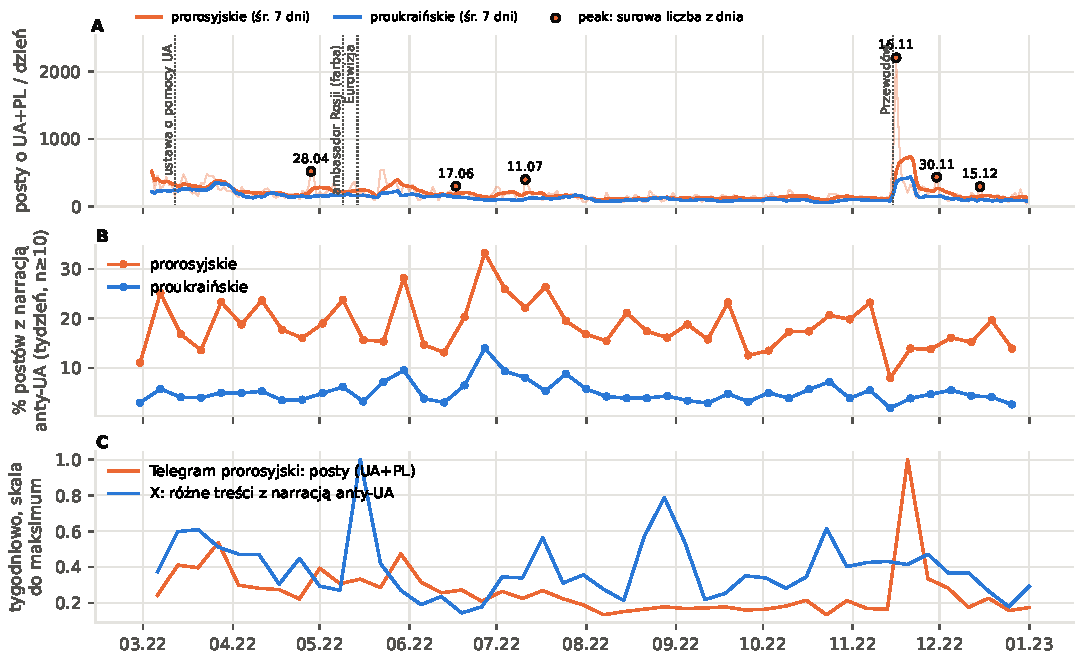
\includegraphics[width=0.8\linewidth]{figures/telegram.pdf}\par}
{\footnotesize\textbf{Rys. 2.} A: dzienna liczba postów według strony (linie: średnia 7 dni; cienka linia i kropki: surowa liczba w kanałach prorosyjskich; kropkowane: wydarzenia z listy); B: tygodniowy udział narracji anty-UA; C: zestawienie wzrokowe tygodniowych liczb z Telegramu prorosyjskiego i z X, każda skalowana do swojego maksimum (bez korelacji i bez testu; hipotezy w M1 nie testujemy).\par}
